
\chapter{Trabalhos Correlatos}

Este capítulo apresenta trabalhos acadêmicos e soluções tecnológicas relacionados à proposta deste estudo, com o objetivo de situar o tema no cenário atual e evidenciar lacunas ainda existentes na literatura e na prática. A análise considera abordagens que tratam do planejamento de redes \gls{ftth} baseadas em \gls{pon}, da representação da topologia de rede, da visualização de dados e da avaliação do desempenho óptico.

Os trabalhos selecionados foram organizados em dois grupos para facilitar a análise comparativa. Os primeiros itens correspondem a trabalhos acadêmicos que investigam o planejamento, a gestão, a visualização de redes ópticas e o uso de bibliotecas de grafos sob diferentes perspectivas. Os itens seguintes referem-se a ferramentas e softwares utilizados no mercado, o que permite contrastar abordagens teóricas e soluções práticas. Essa organização contribui para uma análise mais abrangente e para a identificação de convergências e limitações relevantes.

\section{Projeto e documentação de redes \gls{ftth} com uso de \gls{gis} e AutoCAD \cite{irjet2017ftth_gis_autocad}}

\citeonline{irjet2017ftth_gis_autocad} apresentam uma abordagem voltada ao projeto e à implementação de redes \gls{ftth} com apoio de ferramentas como \gls{gis} e AutoCAD. O estudo destaca procedimentos práticos relacionados à definição do traçado físico e à organização da infraestrutura, contribuindo especialmente para o entendimento da distribuição espacial dos componentes da rede. 

Como limitação, observa-se que a abordagem privilegia a dimensão física do projeto, com ênfase na representação geográfica dos ativos. A estrutura lógica da rede e a avaliação do desempenho do enlace não são exploradas de forma integrada, o que restringe o suporte ao planejamento técnico do sistema como um todo.


\section{Planejamento de redes \gls{ftth} com apoio de \gls{gis} \cite{rezgui2022qgis_ftth}}

\citeonline{rezgui2022qgis_ftth} investigam o uso do QGIS\footnote{O QGIS é um software de sistema de informação geográfica de código aberto, utilizado para visualizar, editar e analisar dados georreferenciados.} para o planejamento de redes \gls{ftth}, evidenciando o potencial das ferramentas de informação geográfica na organização espacial da infraestrutura e no mapeamento de rotas.

Embora a abordagem contribua para o entendimento territorial da rede, a modelagem permanece fortemente vinculada ao espaço geográfico, o que torna secundária a hierarquia lógica característica das arquiteturas \gls{pon}, especialmente o encadeamento entre \gls{olt}, \textit{splitters} e \glspl{onu}. Além disso, não há integração com mecanismos de avaliação do desempenho do enlace, o que limita a análise técnica do projeto.

\section{Gestão de redes \gls{ftth} com análise espacial e monitoramento por \gls{gis}  \cite{chakali2025gis_ftth}}

\citeonline{chakali2025gis_ftth} propõem uma solução baseada em \gls{gis} voltada à gestão de redes \gls{ftth}, integrando análise espacial, banco de dados geográfico e monitoramento de falhas. O trabalho amplia o escopo de aplicação de ferramentas computacionais ao abordar a operação e manutenção da infraestrutura. 

No entanto, o foco concentra-se na fase operacional da rede já implantada. Aspectos associados ao dimensionamento inicial, como definição estrutural da topologia e análise de viabilidade técnica, não constituem o núcleo da abordagem, evidenciando seu direcionamento para gestão e não para planejamento. Dessa forma, a ferramenta proposta neste estudo atua justamente na etapa anterior à gestão operacional, concentrando-se na validação técnica e no apoio ao planejamento que precedem a implantação da infraestrutura.

\section{Visualização interativa da topologia \gls{ftth} em ambiente web \cite{fatahillah2025visnetwork_ftth}}

\citeonline{fatahillah2025visnetwork_ftth} desenvolvem um sistema web para visualização interativa da topologia de redes \gls{ftth}, utilizando bibliotecas de grafos para representar relações entre dispositivos. O estudo reforça a importância da representação gráfica no apoio à compreensão de sistemas complexos. Em comparação com essa abordagem, a utilização da biblioteca D3.js na proposta deste trabalho oferece maior flexibilidade para manipulações customizadas dos dados e da interface, favorecendo a construção de visualizações mais aderentes às necessidades específicas do planejamento lógico de redes \gls{pon}. Esse contraste também evidencia a relevância de discutir, ainda que brevemente, o uso de bibliotecas JavaScript de grafos na literatura, especialmente quanto às possibilidades e limitações de integração com cálculos técnicos em tempo real.

Apesar do avanço na dimensão visual, a proposta não incorpora processos de avaliação técnica associados à transmissão óptica. Dessa forma, a ferramenta atua essencialmente na representação estrutural da rede, sem contemplar a análise do comportamento do enlace e o cálculo automatizado do orçamento de potência óptica.


\section{Visualização de topologias de redes com bibliotecas de grafos em JavaScript}

Diversos estudos na área de visualização de dados exploram o uso de bibliotecas JavaScript para a representação de grafos e redes complexas, com foco na interatividade e na manipulação dinâmica das estruturas apresentadas. Nesse contexto, destacam-se ferramentas como D3.js, Cytoscape.js e outras bibliotecas web utilizadas na construção de diagramas do tipo \textit{node-link}, amplamente aplicados na análise de redes sociais, biológicas e de informação. A biblioteca D3.js, em particular, tem sido reconhecida na literatura por sua capacidade de vincular dados diretamente aos elementos do documento e permitir a construção de visualizações altamente customizáveis, conforme apresentado por \citeonline{bostock2011d3}.

Apesar dos avanços proporcionados por essas bibliotecas, observa-se que grande parte das aplicações descritas na literatura concentra-se na representação visual das redes, com ênfase na disposição espacial dos nós, na interação do usuário e na análise estrutural dos grafos. Em geral, essas soluções são direcionadas à exploração visual e à navegação sobre estruturas relacionais, sem integração direta com modelos matemáticos ou cálculos técnicos específicos do domínio da aplicação. Assim, embora sejam eficazes para fins de visualização, apresentam limitações quando se trata da incorporação de cálculos especializados realizados de forma dinâmica e integrada à interface gráfica.

No contexto do planejamento de redes ópticas, especialmente em arquiteturas \gls{pon}, não foram identificados, na literatura analisada, trabalhos que integrem de forma direta a modelagem visual interativa da topologia com o cálculo automatizado do orçamento óptico em tempo real. Essa lacuna evidencia uma oportunidade de contribuição, uma vez que o uso do D3.js permite não apenas a construção de representações visuais interativas, mas também a manipulação direta dos dados associados aos elementos da rede. Dessa forma, a abordagem proposta neste trabalho diferencia-se das soluções puramente visuais ao integrar, em uma mesma aplicação, a visualização dinâmica da topologia e a análise técnica do enlace, proporcionando maior suporte ao processo de planejamento de redes ópticas.


\section{Plataforma georreferenciada para documentação de redes ópticas (GeoGrid Maps)}

O GeoGrid Maps é uma plataforma voltada à documentação e ao gerenciamento de redes de fibra óptica, oferecendo recursos de mapeamento georreferenciado, cadastro de infraestrutura e análise operacional da rede \cite{geogridmaps2026,geogrid_iclass_2026}. A ferramenta representa uma tendência de mercado que busca integrar inventário e gestão em um único ambiente. 

A Figura~\ref{fig:geogrid_mapa} ilustra a abordagem predominante desse tipo de solução, na qual a rede é representada com ênfase na localização geográfica dos elementos, evidenciando rotas, conexões físicas e distribuição espacial dos ativos. Nesse modelo, a visualização privilegia ``onde'' os componentes estão posicionados, facilitando atividades de documentação, operação e manutenção da infraestrutura. 

\begin{figure}[htb]
	\caption{Visualização georreferenciada da rede, destacando a localização dos elementos}
	\label{fig:geogrid_mapa}
    \centering
    \parbox{16cm}{
		\centering
		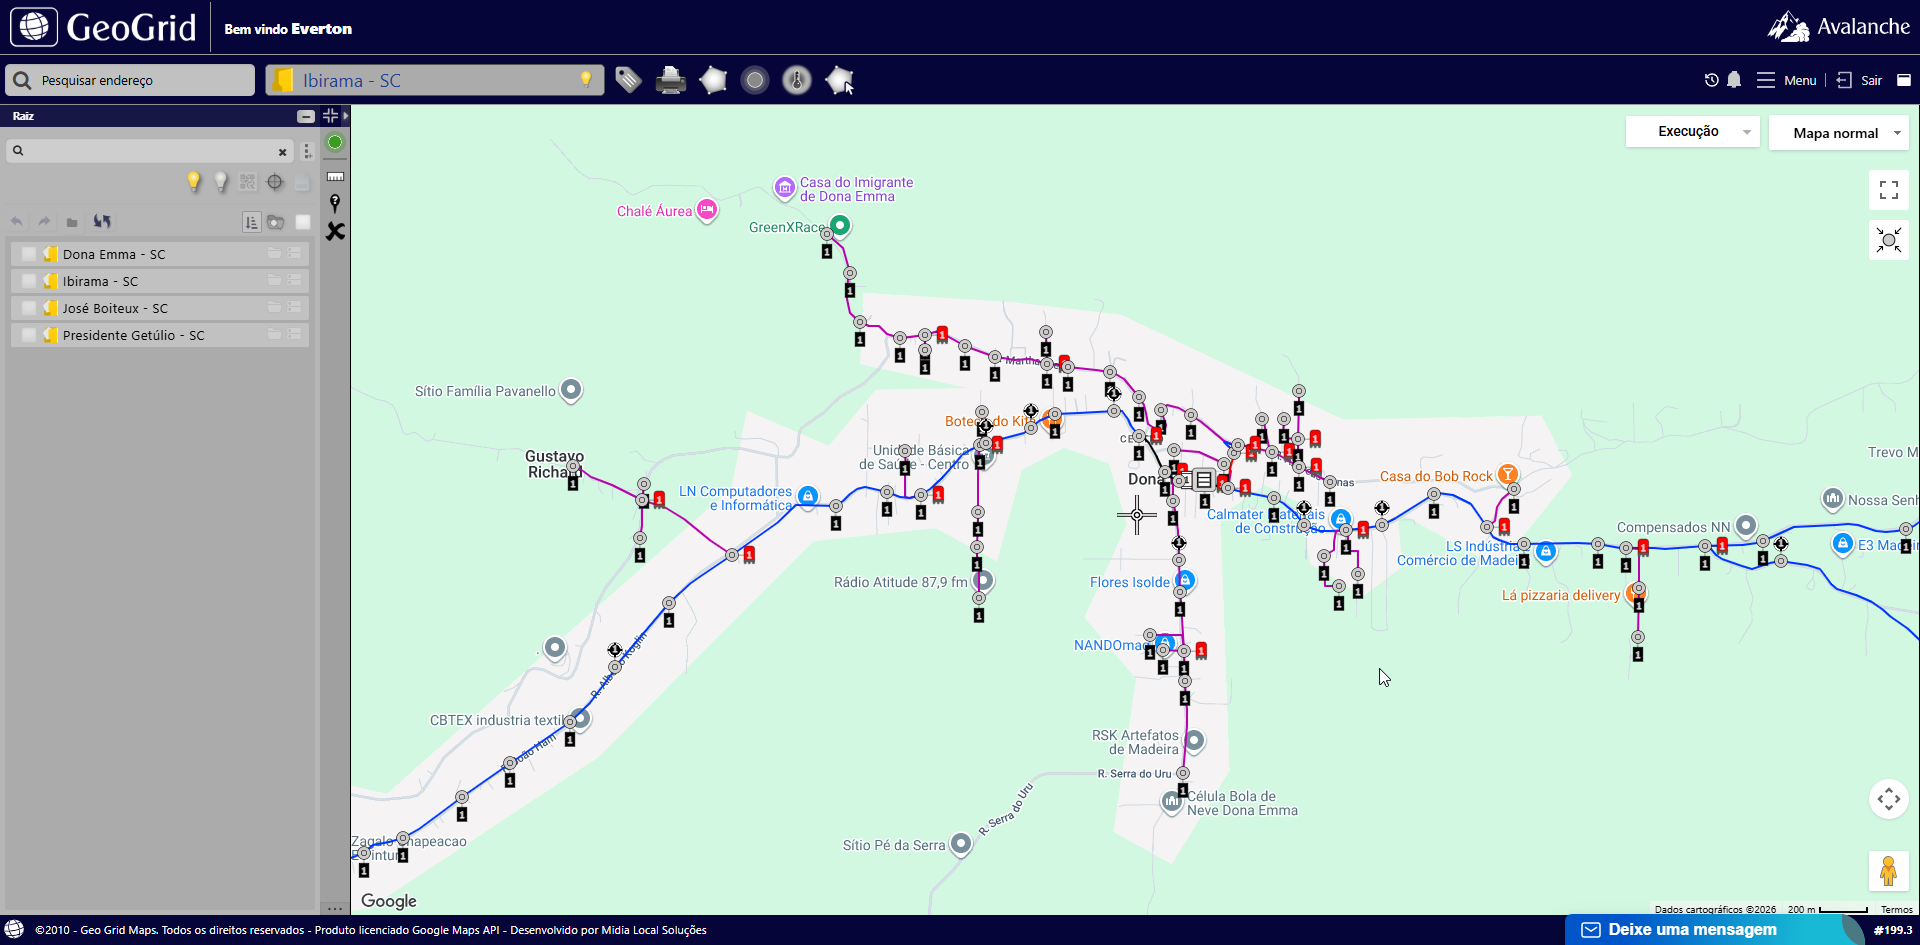
\includegraphics[width=\textwidth]{images/geogrid_mapa.png}
		\par\footnotesize Fonte: Adaptado da ferramenta GeoGrid Maps.
    }
\end{figure}

Adicionalmente, a Figura~\ref{fig:geogrid_ceo} exemplifica a representação detalhada de elementos internos da rede, como fusões em caixas de emenda, reforçando o caráter descritivo e cadastral dessas ferramentas, voltado à organização física dos componentes da rede óptica. 

\begin{figure}[htb]
	\caption{Detalhamento de fusões numa caixa de emenda}
	\label{fig:geogrid_ceo}
    \centering
    \parbox{16cm}{
		\centering
		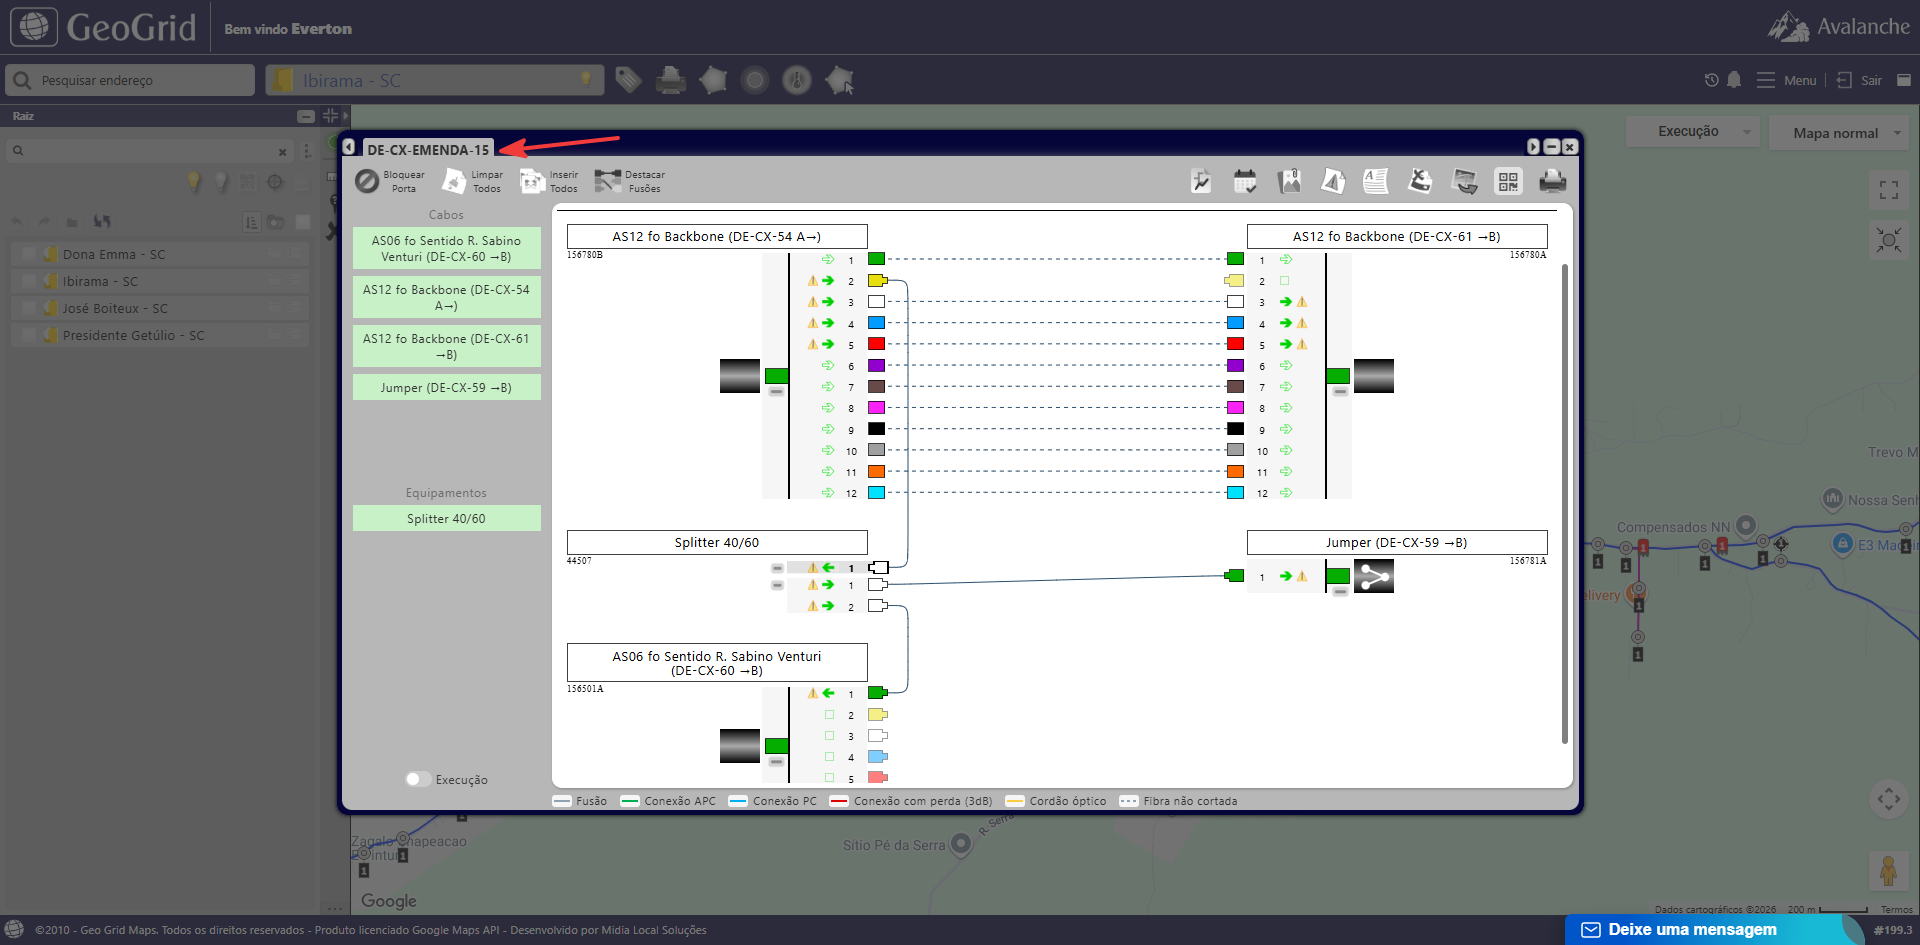
\includegraphics[width=\textwidth]{images/geogrid_ceo.png}
		\par\footnotesize Fonte: Adaptado da ferramenta GeoGrid Maps.
    }
\end{figure}

Apesar de sua relevância no contexto operacional, esse tipo de abordagem não atende plenamente ao problema tratado neste trabalho. Isso ocorre porque o foco permanece na representação geográfica e na documentação dos ativos, não contemplando de forma central a modelagem lógica da topologia da rede nem a análise integrada do orçamento óptico ao longo do enlace. Em geral, ferramentas dessa natureza funcionam sobretudo como repositórios estruturados de dados da rede: permitem cadastrar, organizar, consultar e visualizar informações sobre a infraestrutura implantada, mas tendem a pressupor que o usuário já possua o conhecimento técnico necessário para interpretar os parâmetros do projeto e realizar, por conta própria, os cálculos de validação do enlace. Dessa forma, embora essas soluções sejam adequadas para inventário, gestão e apoio à operação da rede implantada, elas não oferecem suporte direto à geração do conhecimento técnico associado ao planejamento lógico e à verificação automatizada da viabilidade óptica. Em contraste, a proposta desenvolvida neste trabalho busca justamente integrar a modelagem visual da rede à produção desse conhecimento técnico, por meio do cálculo automático do orçamento óptico, apoiando de forma mais direta o processo de planejamento e validação do enlace.

\section{Ferramenta de mapeamento e inventário de redes FTTx (OZmap)}

O OZmap é amplamente utilizado para mapeamento e documentação de redes FTTx, permitindo o cadastro e a visualização de elementos como cabos, caixas e clientes em ambiente georreferenciado \cite{ozmap2026,ozmap_help_2025}. A ferramenta destaca-se pela capacidade de organizar a infraestrutura e apoiar atividades de expansão e manutenção. 

A Figura~\ref{fig:ozmap_mapa} exemplifica a abordagem adotada por esse tipo de solução, na qual a rede é representada com base na sua distribuição geográfica. Observa-se que a visualização enfatiza a localização dos elementos no mapa, permitindo identificar rotas, posicionamento de caixas e distribuição da infraestrutura ao longo do território. Essa característica é particularmente útil para fins de inventário e operação da rede. 

\begin{figure}[htb]
	\caption{Visualização georreferenciada da rede no OZmap}
	\label{fig:ozmap_mapa}
    \centering
    \parbox{16cm}{
		\centering
		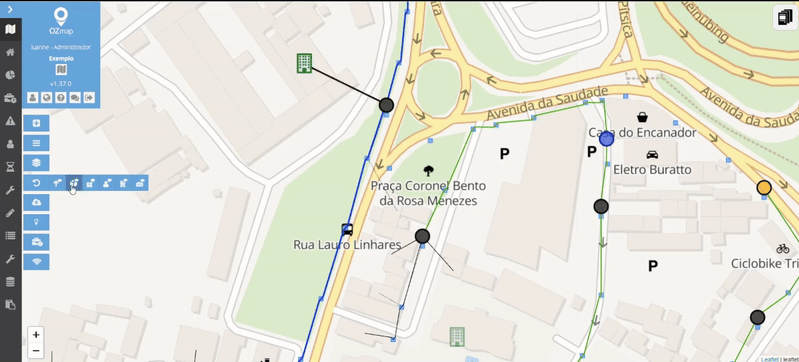
\includegraphics[width=\textwidth]{images/ozmap_mapa.png}
		\par\footnotesize Fonte: Adaptado da documentação do OZmap.
    }
\end{figure}

Além disso, esse modelo de visualização tende a dificultar a análise da estrutura lógica da rede, especialmente no contexto de arquiteturas \gls{pon}. Conforme ilustrado na Figura~\ref{fig:ozmap_diagrama}, a representação simultânea de múltiplos elementos, conexões e ramificações em um ambiente geográfico pode resultar em diagramas visualmente densos, com excesso de informações e baixa legibilidade da topologia de ponta a ponta. Essa sobreposição de elementos no espaço cartográfico pode gerar sobrecarga cognitiva, dificultando a percepção da continuidade lógica do sinal ao longo da rede e a compreensão clara do encadeamento entre seus componentes.

\begin{figure}[htb]
	\caption{Representação da rede com múltiplos elementos e alto nível de complexidade visual}
	\label{fig:ozmap_diagrama}
    \centering
    \parbox{16cm}{
		\centering
		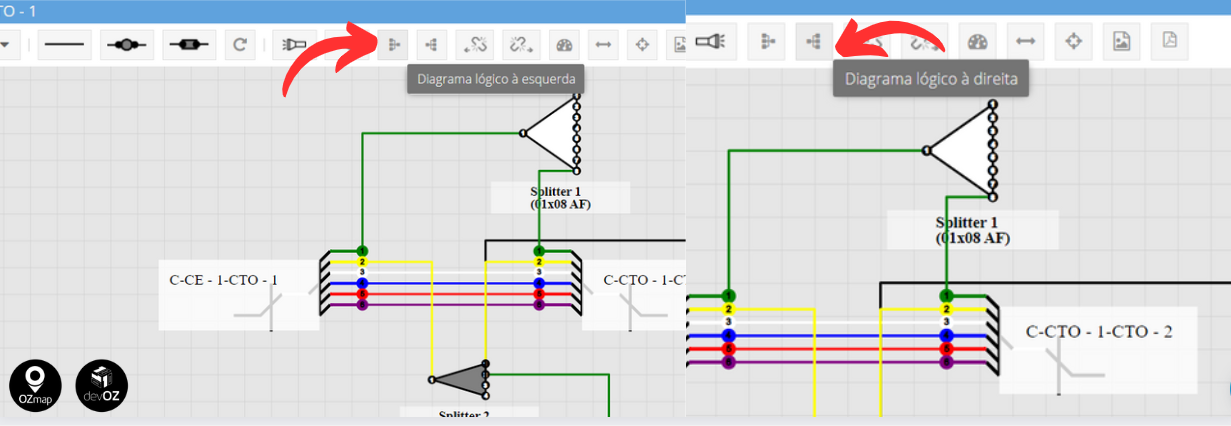
\includegraphics[width=\textwidth]{images/ozmap_diagrama.png}
		\par\footnotesize Fonte: Adaptado da documentação do OZmap.
    }
\end{figure}

Embora ferramentas como o OZmap sejam eficazes para documentação e gestão da rede implantada, elas não atendem plenamente ao problema abordado neste trabalho. Isso ocorre porque não oferecem uma representação orientada à compreensão lógica da topologia nem integram, de forma central, o cálculo do orçamento óptico ao processo de visualização. 

A limitação dessas soluções reside na dificuldade de apoiar o planejamento técnico do enlace, no qual é necessário compreender claramente a hierarquia da topologia ponto-multiponto e avaliar a viabilidade da transmissão óptica ao longo de toda a rede.


\section{Ferramenta de planejamento e documentação \gls{ftth} (FTTH Planner)}

O FTTH Planner apresenta-se como uma ferramenta voltada ao planejamento e à documentação de redes \gls{ftth}, oferecendo recursos para organização da infraestrutura e visualização de elementos em ambiente georreferenciado \cite{ftthplanner2026}. 

A Figura~\ref{fig:planner_mapa} ilustra a representação da rede com base na sua distribuição geográfica, evidenciando a localização dos elementos ao longo do território. Essa abordagem permite identificar rotas, posicionamento de caixas e organização da infraestrutura, sendo adequada para fins de planejamento físico e documentação da rede. 

\begin{figure}[htb]
	\caption{Visualização georreferenciada da rede no FTTH Planner}
	\label{fig:planner_mapa}
    \centering
    \parbox{16cm}{
		\centering
		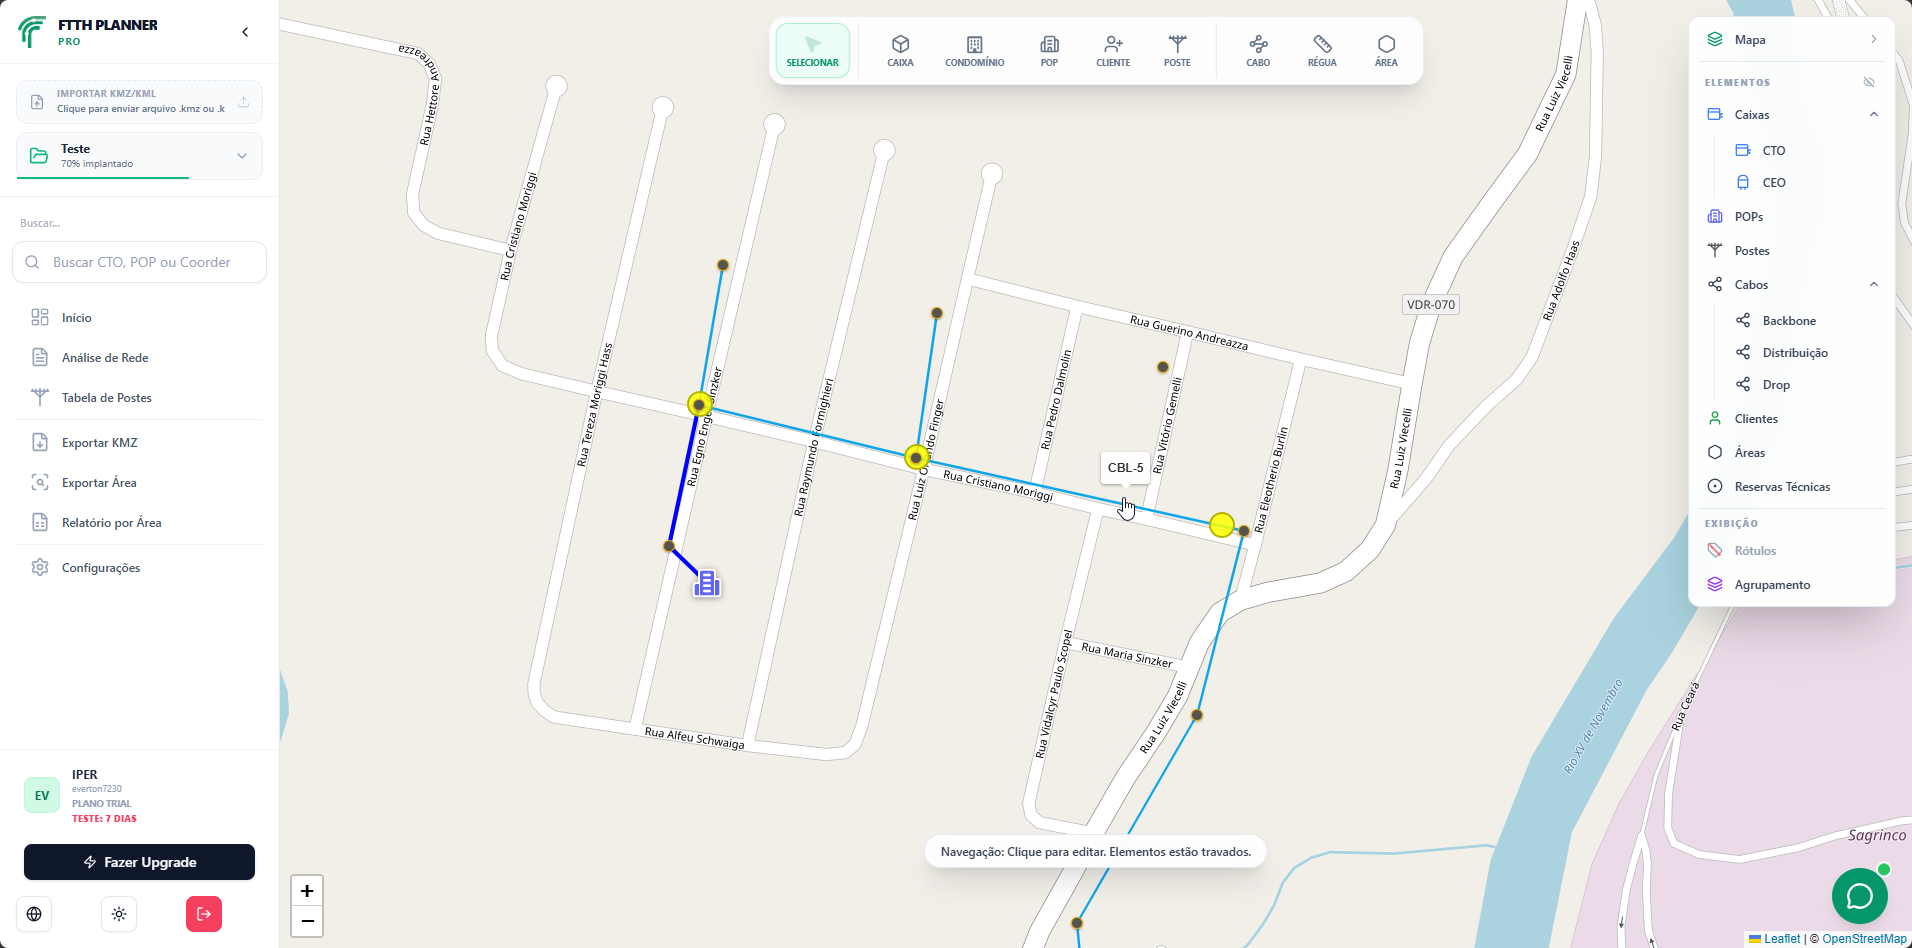
\includegraphics[width=\textwidth]{images/planner_mapa.png}
		\par\footnotesize Fonte: Adaptado do FTTH Planner.
    }
\end{figure}

Adicionalmente, a Figura~\ref{fig:planner_ceo} apresenta a visualização de fusões em caixas de emenda, destacando a forma como a ferramenta representa conexões internas da rede em nível local. Esse tipo de diagrama facilita a análise pontual de componentes específicos, especialmente para fins de organização e manutenção. 

\begin{figure}[htb]
	\caption{Representação de fusões em caixa de emenda no FTTH Planner}
	\label{fig:planner_ceo}
    \centering
    \parbox{16cm}{
		\centering
		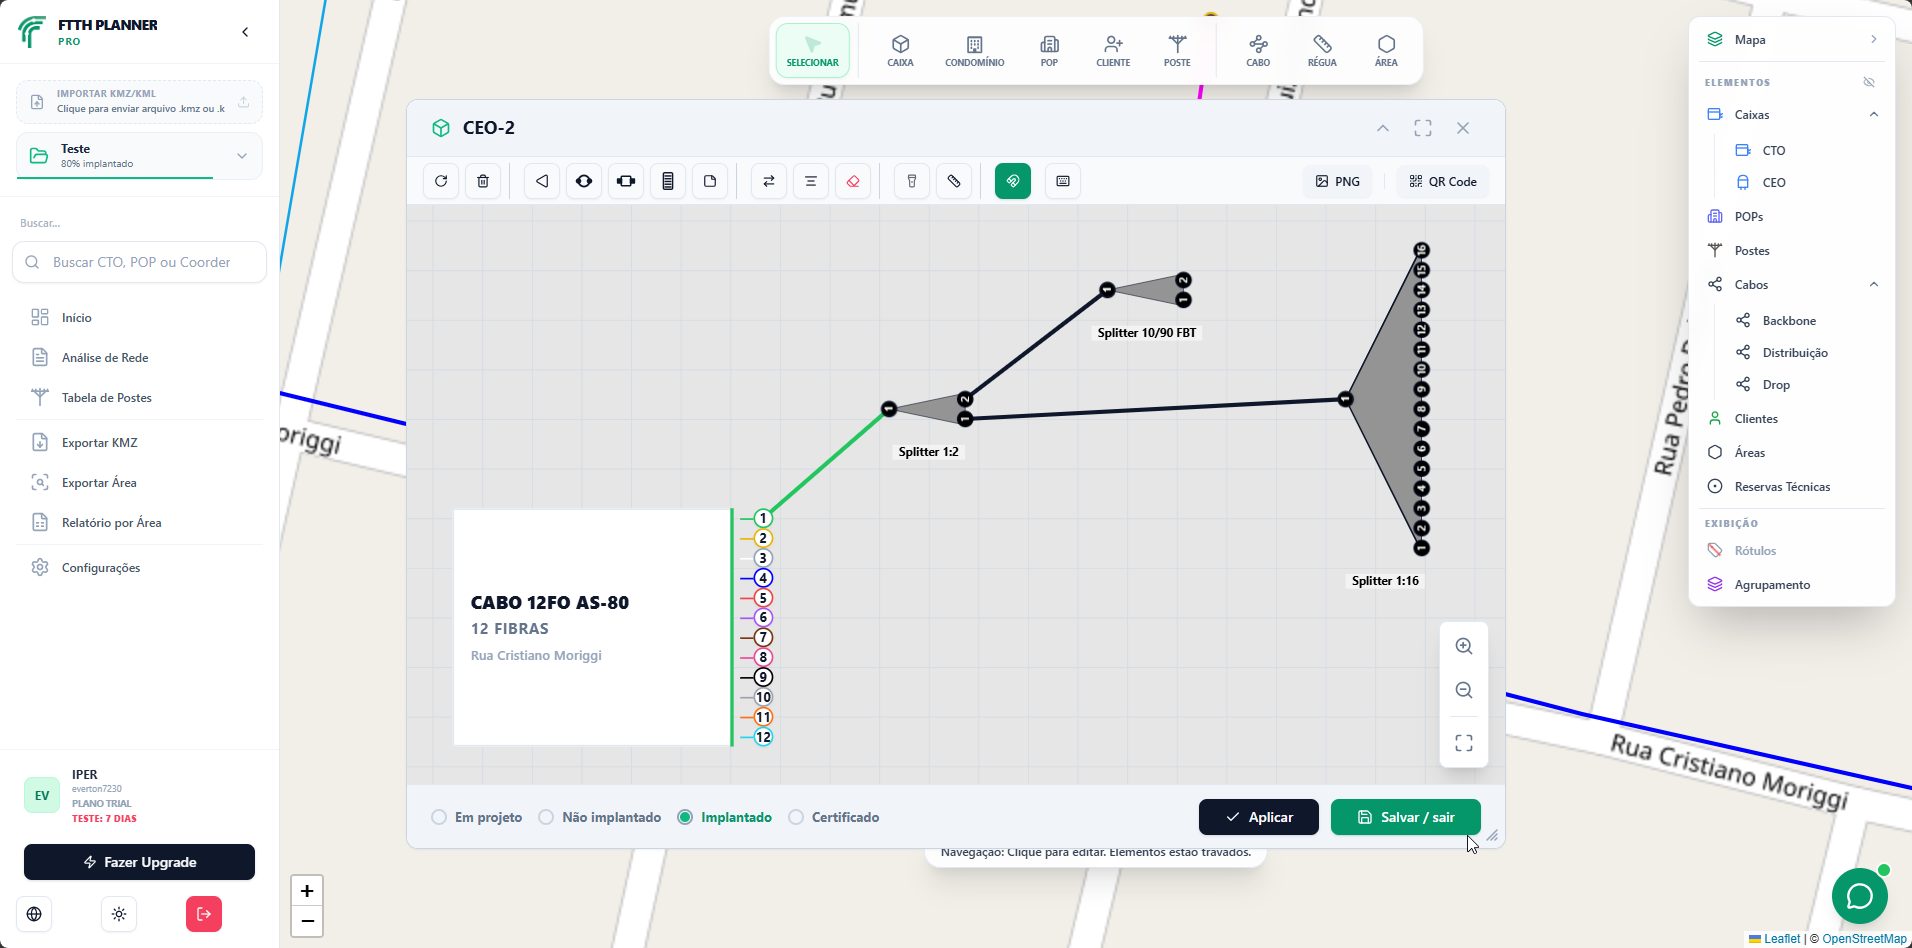
\includegraphics[width=\textwidth]{images/planner_ceo.png}
		\par\footnotesize Fonte: Adaptado do FTTH Planner.
    }
\end{figure}

A ferramenta não disponibiliza mecanismos para modelagem lógica completa da topologia da rede nem para o cálculo do orçamento óptico ao longo do enlace. A representação permanece concentrada na localização geográfica dos elementos e na visualização isolada de conexões em caixas, sem oferecer uma visão integrada do encadeamento da rede desde a origem até os pontos finais. 

Embora contribua para o registro e a organização da infraestrutura, o FTTH Planner não atende plenamente ao problema abordado neste trabalho, uma vez que não permite a análise conjunta da topologia lógica e do orçamento óptico. Essa limitação dificulta a validação técnica do projeto, a compreensão global do comportamento do enlace e a identificação de possíveis gargalos de potência ao longo da rede, aspectos centrais para o planejamento e a tomada de decisão técnica. Nesse sentido, a visão integrada proposta neste estudo amplia a utilidade prática da ferramenta ao apoiar não apenas a documentação da infraestrutura, mas também a análise da viabilidade óptica e a detecção antecipada de pontos críticos do enlace.


\section{Análise Comparativa}

De forma geral, os trabalhos acadêmicos revisados demonstram avanços importantes em aspectos específicos do planejamento de redes \gls{ftth}, como análise espacial, visualização de dados e gestão da infraestrutura. No entanto, esses aspectos são frequentemente tratados de maneira isolada, sem integração entre a modelagem da topologia lógica, a visualização interativa e o cálculo do orçamento óptico. 

As ferramentas de mercado, por sua vez, evidenciam a demanda prática por soluções integradas, especialmente no contexto de documentação e operação da rede. Ainda assim, a maioria delas privilegia o inventário e a gestão geográfica, com menor ênfase na análise técnica estruturada do enlace. 

A principal lacuna identificada não é a ausência de soluções, mas a falta de integração entre os elementos fundamentais discutidos na fundamentação teórica: representação visual da topologia, cálculo automatizado do orçamento óptico e apoio ao processo de planejamento. As Tabelas~\ref{tab:comparativo_trabalhos} e \ref{tab:comparativo_ferramentas} sintetizam essa leitura comparativa.

\begin{table}[htb]
    \centering
    \caption{Comparação entre trabalhos acadêmicos correlatos}
    \label{tab:comparativo_trabalhos}
    \small
    \begin{tabularx}{\textwidth}{|p{3.0cm}|X|c|c|X|}
        \hline
        \textbf{Trabalho} & \textbf{Foco principal} & \textbf{Vis. lógica} & \textbf{Cálculo óptico} & \textbf{Limitação principal} \\
        \hline
        Lokhande e Singh (2017) & Projeto físico de rede FTTH com GIS e AutoCAD & Não & Não & Ênfase no projeto físico da rede \\
        \hline
        Rezgui e Bourezg (2022) & Planejamento FTTH com apoio do QGIS & Parcial & Não & Foco espacial e documental \\
        \hline
        Chakali et al. (2025) & Gestão de rede com GIS e monitoramento de falhas & Parcial & Não & Ênfase em operação e manutenção \\
        \hline
        Fatahillah e Wulandari (2025) & Visualização web da topologia FTTH/OLT & Sim & Não & Não integra orçamento óptico \\
        \hline
        Proposta deste trabalho & Planejamento lógico de redes PON com apoio visual & Sim & Sim & Integra visualização, cálculo e persistência \\
        \hline
    \end{tabularx}
\end{table}

\begin{table}[htb]
    \centering
    \caption{Comparação entre ferramentas e softwares correlatos}
    \label{tab:comparativo_ferramentas}
    \small
    \begin{tabularx}{\textwidth}{|p{3.0cm}|X|c|c|X|}
        \hline
        \textbf{Ferramenta} & \textbf{Foco principal} & \textbf{Vis. lógica} & \textbf{Cálculo óptico} & \textbf{Limitação principal} \\
        \hline
        GeoGrid Maps & Documentação de rede e apoio operacional para provedores & Parcial & Parcial & Ênfase operacional e geográfica \\
        \hline
        OZmap & Mapeamento e documentação georreferenciada de redes FTTx & Parcial & Não central & Foco cartográfico e operacional \\
        \hline
        FTTH Planner & Registro de elementos georreferenciados e inventário & Parcial & Não & Ausência de cálculo integrado e foco geográfico \\
        \hline
        Proposta deste trabalho & Planejamento lógico de redes PON com apoio visual & Sim & Sim & Integra visualização, cálculo e persistência em contexto acadêmico\\
        \hline
    \end{tabularx}
\end{table}

\section{Posicionamento da Proposta}

Com base na análise dos correlatos, observa-se que a proposta deste trabalho se posiciona na interseção entre planejamento técnico de redes \gls{pon}, visualização de dados e desenvolvimento de aplicações web, com foco na integração desses elementos em um ambiente único. 

Diferentemente dos trabalhos acadêmicos analisados, que tendem a abordar isoladamente o planejamento geográfico, a visualização ou a gestão da rede, a proposta integra a modelagem visual interativa da topologia ponto-multiponto com o cálculo automatizado do orçamento óptico. Em relação às ferramentas de mercado, o foco desloca-se da documentação e operação para o apoio ao planejamento técnico, priorizando a compreensão lógica do enlace e a validação das decisões de projeto. 

A Figura~\ref{fig:diagrama_proposta} apresenta uma representação conceitual da abordagem proposta neste trabalho. O diagrama ilustra, de forma simplificada, a estrutura de uma rede óptica e os principais elementos que compõem o cálculo do orçamento óptico, até os terminais finais, bem como as perdas acumuladas ao longo do enlace. Essa representação, embora preliminar, auxilia na compreensão do objetivo da ferramenta a ser desenvolvida, destacando a integração entre a modelagem da topologia e a análise dos parâmetros técnicos da rede. 

\begin{figure}[htb]
	\caption{Representação conceitual da rede óptica e do cálculo do orçamento óptico}
	\label{fig:diagrama_proposta}
    \centering
    \parbox{16cm}{
		\centering
		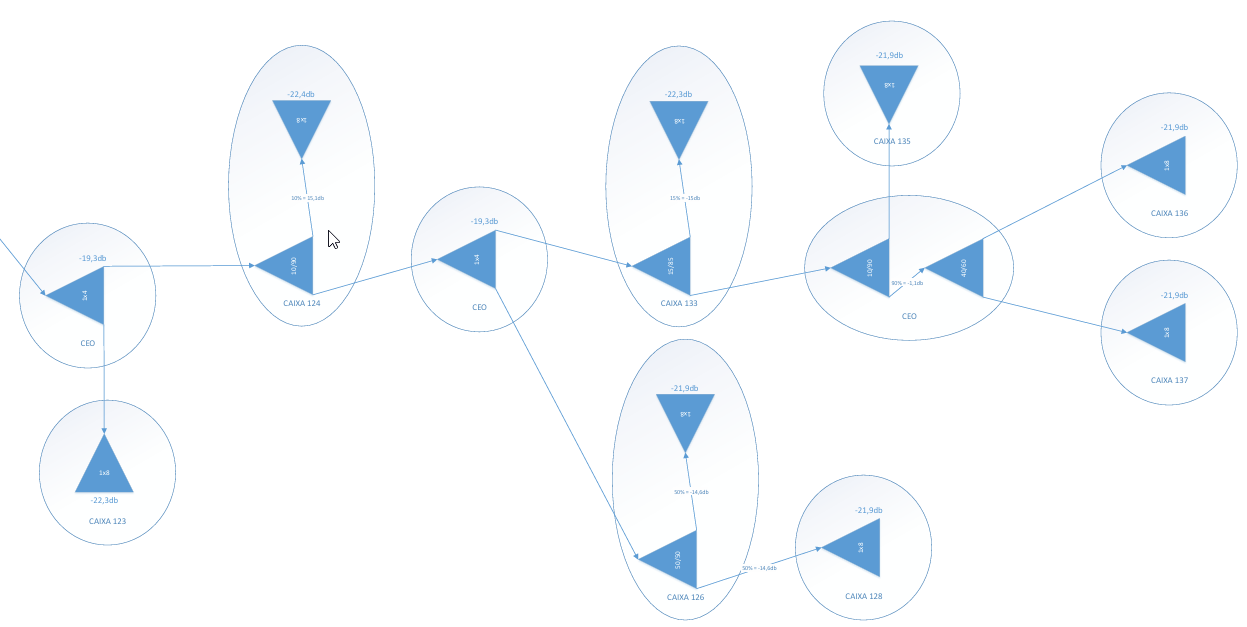
\includegraphics[width=\textwidth]{images/diagrama_proposta.png}
		\par\footnotesize Fonte: Elaboração própria.
    }
\end{figure}

Assim, a contribuição do trabalho não reside apenas na utilização de tecnologias conhecidas, mas na articulação entre seus componentes para atender a uma lacuna específica: a integração entre visualização, cálculo e modelagem da rede.
